\chapter{Bewertung}

Das Ergebnis der Arbeit ist ein innovatives, funktionstüchtiges Werkzeug, das in der Lage ist dem
Nutzer bei der Arbeit mit Beweisdokumenten eine sinnvolle und produktive Unterstützung zu gewähren.
Als Maßstab für die Einordnung der Ergebnisse bietet sich ein Vergleich mit dem bisherigen Ansatz
Isabelle/jEdit an. 

Dabei ist allerdings zu beachten, dass es sich bei diesem Projekt auch um eine Machbarkeitsstudie
für die Umsetzung einer webbasierten IDE handelt, da es nicht möglich ist eine sogenannte
\textit{full featured} IDE im Rahmen einer Diplomarbeit zu entwickeln und dabei noch die vielen
neuen Aspekte im Zusammenhang mit der Kommunikation einer Webanwendung zu beachten.

\section{Funktionalität}

Ein klarer Nachteil gegenüber dem Proof General ist die fehlende Möglichkeit der
\textbf{semantischen Suche} in Isabelle Quellen. Diese Funktionalität wird von der Isabelle
Plattform bereit gestellt und ist bis jetzt leider von der Isabelle/Scala Schnittstelle noch nicht
unterstützt (Und daher auch in Isabelle/jEdit nicht vorhanden).

Darüber hinaus fehlt natürlich die Infrastruktur an Plugins welche für jEdit existiert, da es sich
bei der Anwendung notwendiger Weise um eine Neuentwicklung handelt. Das macht es natürlich mühsamer
zusätzliche Funktionalität, wie Versionsverwaltungssystem oder andere Erweiterungen, zu integrieren,
da diese dann speziell für diese neue Plattform entwickelt werden müssen.

Eine große Zahl von Funktionen ist nur über Tastenkürzel verfügbar, jedoch nicht über Mausaktionen,
diese Nachzurüsten ist eher Fleißarbeit, da die Infrastruktur für Kommandos in der Sidebar bereits
fertiggestellt wurde. Dieser Umstand betrifft damit eher die Usability in
Abschnitt\,\ref{sec:usability}.

\section{Zuverlässigkeit}

Da die Browseranwendung zwingender Weise in \acr{js}, also einer dynamischen Sprache entwickelt
werden musste ist es schwieriger, Fehler zu entdecken, da Typfehler in sprachen mit dynamischer
Typisierung logischerweise nicht existieren und der Compiler so keine große Hilfe bei der
Fehlerfindung darstellt. Während der Entwicklung wurden sogenannte \textit{cross checks} im Code
geführt (Welche nun auskommentiert sind (Siehe z.B. \texttt{isabelle.coffee})) um die
Datenkonsistenz regelmäßig zu überprüfen. Das reicht aber natürlich nicht aus um die Fehlerfreiheit
zu garantieren und da darüber hinaus das systematische Testen von Benutzeroberflächen immer ein
Problem darstellt, kann nicht ausgeschlossen werden, dass sich noch Fehler in der
Benutzerschnittstelle befinden.

Serverseitig mussten vor allem der \texttt{LineBuffer} und das \texttt{RemoteDocumentModel} getestet
werden. Hierfür wurde zum einen eine zuschaltbare Visualisierung der Serverseitigen Daten
implementiert sowie einige in ScalaTest implementierte Testfälle (\texttt{/test/scala/...}). Die
meiste andere Funktionalität stammt aus Isabelle/Scala bzw. Play und wurde nur verknüpft.

\section{Benutzbarkeit}
\label{sec:usability}

Da es sich um eine Benutzerschnittstelle handelt ist Usability ein wichtiges Thema. Leider ist dies
bei der Konzeption zu kurz gekommen. Da es sich um eine Machbarkeitsstudie handelt, wurden einige
Aspekte der Usability zunächst hinten angestellt. Insbesondere auch die Barrierefreiheit, da diese
in einer \textit{single-page}-HTML-Anwendung bislang schwer zu erreichen ist, nicht zuletzt auch
weil viele unkonventionelle ELemente verwendet werden mussten. Anstelle von ausgiebigen Usability
Tests wurde die Anwendung einigen Probanden (Kommilitonen) zur Benutzung vorgelegt, und deren
Verhalten beobachtet. Dabei wurden einige Lücken gewahr, die noch geschlossen werden konnten. So
wurden beispielsweise nach den Tests die meisten Kommandos auf Standard Tastenkombinationen gelegt.

Isabelle/jEdit hat hier natürlich den Vorteil, dass es in einer ausgereiften Umgebung (jEdit) lebt,
die über einige hundert Personenjahre Entwicklungszeit entstanden ist und damit in den Details viel
vielfältiger und komfortabler für den Nutzer ist.

\section{Performanz}

Da die selbe Bibliothek (Isabelle/Scala) zu Grunde liegt, gibt es keine Unterschiede in der
Geschwindigkeit des Beweisers selbst. Bei der lokalen Ausführung auf einem Rechner mit Server und
Browser ist zu erwarten, dass es durch die Kommunikation über Serialisierte Nachrichten und deren
Umrechnung zu leichten Geschwindigkeitseinbußen gegenüber Isabelle/jEdit kommt. Die Performanz auf
diese Weise zu vergleichen is jedoch nicht sinnvoll, da in einem normalen Szenario der Server auf
einem zentralen Rechner ausgeführt wird, der über die nötigen Ressourcen verfügt um die Isabelle
Plattform tragen zu können. Der Zugriff geschieht dann über mehrere Clients die keine besonders
hohen Ansprüche erfüllen müssen. Hier liegt ein Vorteil gegenüber der jEdit Implementierung.
Mit \textit{clide} ist es theoretisch möglich einen Theorembeweiser von einem Netbook oder einem
Tablet PC aus zu verwenden.

\section{Visualisierung}

\begin{figure}[ht]
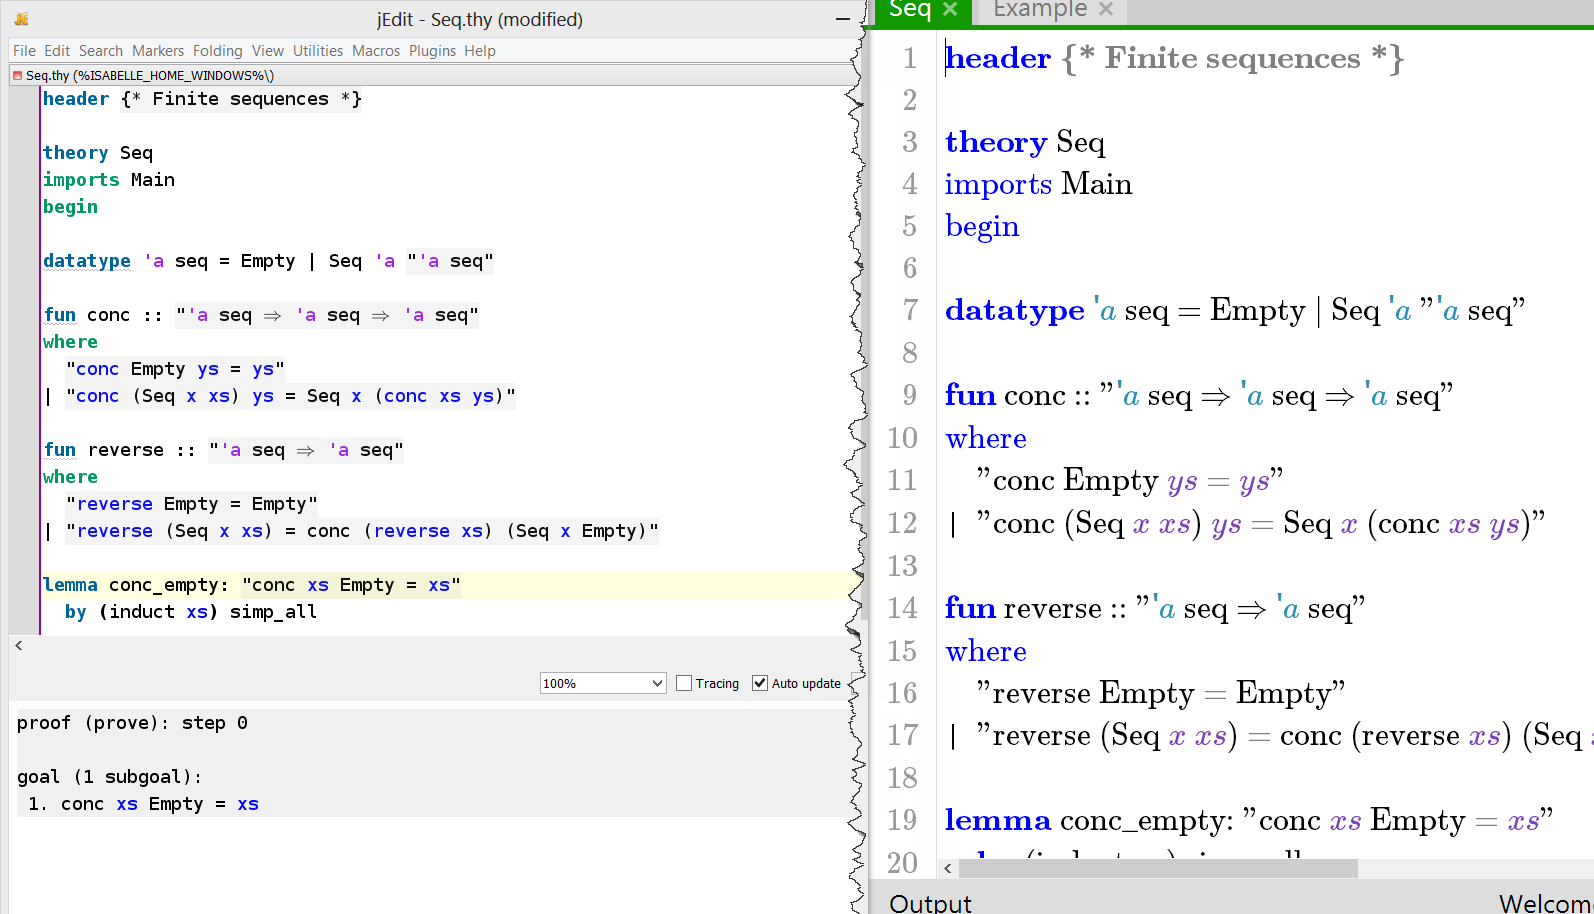
\includegraphics[width=\linewidth]{images/jedit}
  \caption{jEdit vs. clide}
  \label{fig:jedit}
\end{figure}

Hier ist eine klare Verbesserung gegenüber Isabelle/jEdit zu erkennen. Während Isabelle/jEdit sich
am festen Textraster, welches in jEdit vorgegeben ist orientieren musste und nur geringe
Abweichungen implementieren konnte, ähnelt die Darstellung in der Bearbeitung bei der Webanwendung
schon sehr stark der Endgültigen Darstellung in Veröffentlichten LaTeX Dokumenten (Siehe
Abbildung\,\ref{fig:jedit})

Darüber hinaus ist die Integration der Beweiser-Ausgaben flexibler gestaltet und es ist auch möglich
dise teilweise oder vollständig \textit{inline} anzuzeigen.